%%%%%%%%%%%%%%%%%%%%%%%%%%%%%%%%%%%%%%%%%
% Developer CV
% LaTeX Template
% Version 1.0 (28/1/19)
%
% This template originates from:
% http://www.LaTeXTemplates.com
%
% Authors:
% Jan Vorisek (jan@vorisek.me)
% Based on a template by Jan Küster (info@jankuester.com)
% Modified for LaTeX Templates by Vel (vel@LaTeXTemplates.com)
%
% License:
% The MIT License (see included LICENSE file)
%
%%%%%%%%%%%%%%%%%%%%%%%%%%%%%%%%%%%%%%%%%

%----------------------------------------------------------------------------------------
%	PACKAGES AND OTHER DOCUMENT CONFIGURATIONS
%----------------------------------------------------------------------------------------

\documentclass[10pt]{developercv} % 8-12pt recommended
\usepackage[backend=biber, style=authoryear, sorting=ydnt, natbib=true, url=true, doi=false, maxnames=24]{biblatex}
\addbibresource{publications.bib}

%----------------------------------------------------------------------------------------

\begin{document}

%----------------------------------------------------------------------------------------
%	TITLE AND CONTACT INFORMATION
%----------------------------------------------------------------------------------------

\begin{minipage}[t]{0.45\textwidth} % 45% of the page width for name
	\vspace{-\baselineskip} % Required for vertically aligning minipages
	% First name
	\colorbox{black}{{\HUGE\textcolor{white}{\textbf{\MakeUppercase{Brendan}}}}} 
	% Last name
	\colorbox{black}{{\HUGE\textcolor{white}{\textbf{\MakeUppercase{Harmon }}}}} 
	
\end{minipage}
\begin{minipage}[t]{0.275\textwidth}
	\vspace{-\baselineskip} 
%	\icon{MapMarker}{12}{Baton Rouge}\\
	\icon{At}{12}{\href{mailto:baharmon@lsu.edu}{baharmon@lsu.edu}}\\
	\icon{Phone}{12}{1 919 622 8414}\\
	
\end{minipage}
\begin{minipage}[t]{0.275\textwidth}
	\vspace{-\baselineskip}
	\icon{Globe}{12}{\href{https://baharmon.github.io}{baharmon.github.io}}\\	
	\icon{Github}{12}{\href{https://github.com/baharmon}{github.com/baharmon}}\\
%	\aicon{Orcid}{12}{\href{https://orcid.org/0000-0002-6218-9318}{0000-0002-6218-9318}}\\
%	\aicon{ResearchGate}{12}{\href{https://www.researchgate.net/profile/Brendan\_Harmon2/}{Brendan\_Harmon2}}\\
%	\aicon{OSF}{12}{\href{https://osf.io/xhvp4/}{osf.io/xhvp4}}\\
\end{minipage}

\vspace{16pt}

{\huge Assistant Professor of Landscape Architecture \par} 

\vspace{8pt}


\includegraphics[width=6cm]{images/lsu_art_design_logo.pdf}


%----------------------------------------------------------------------------------------
%	INTRODUCTION, SKILLS AND TECHNOLOGIES
%----------------------------------------------------------------------------------------
\begin{minipage}[t]{0.35\textwidth}
\cvsect{About} %Who Am I?
\newline
\end{minipage}
\hfill
\begin{minipage}[t]{0.2\textwidth}
\end{minipage}
\hfill
\begin{minipage}[t]{0.35\textwidth}
\cvsect{Research Interests}
\newline
\end{minipage}

\begin{minipage}[t]{0.35\textwidth}
	\vspace{-\baselineskip}

	I am interested in dynamic landscapes, 
	in modeling how landscapes evolve
	%simulating the processes that shape them,
	and designing catalysts for change. 
	%
	My teaching focuses on how 
	scientific modeling can play a generative role
	in the creative design process.
	%
	My research explores creative applications
	for emerging technologies like tangibles and robotics.

	
%	I teach Geographic Information Systems (GIS),
%	3D modeling, generative design, and digital fabrication.

\end{minipage}
\hfill
\begin{minipage}[t]{0.2\textwidth} 
	\vspace{-\baselineskip} 
	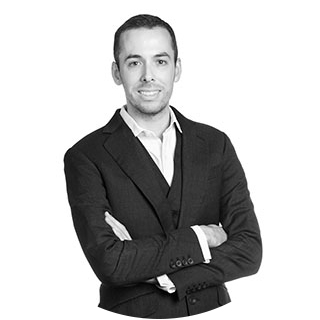
\includegraphics[width=3cm]{images/baharmon-2.jpg}
\end{minipage}
\hfill
\begin{minipage}[t]{0.35\textwidth} 
	\vspace{-\baselineskip} 
				
		\textbf{Geospatial Modeling}
			erosion modeling \textbullet{}
			landscape evolution \textbullet{}
			computational ecology \textbullet{}
			lidar \& drone analytics \textbullet{}
			geovisualization\\
			
		\textbf{Digital Design}
		generative design \textbullet{}
		creative coding \textbullet{}
		digital fabrication \textbullet{}
		ecological robotics \textbullet{}
		human-computer interaction \textbullet{}
		tangible interfaces\\
\end{minipage}

%----------------------------------------------------------------------------------------
%	EDUCATION
%----------------------------------------------------------------------------------------

\cvsect{Education}

\begin{entrylist}
	\entry
		{2013 -- 2017}
		{PhD in Design}
		{North Carolina State University}
		{Co-major in Forestry and Environmental Science}
	\entry
		{2010 -- 2012}
		{Master's of Philosophy in Geography} %\& the Environment
		{University of Oxford}
		{Focus in Biodiversity, Conservation, and Management}
	\entry
		{2005 -- 2008}
		{Master's of Landscape Architecture}
		{Harvard Graduate School of Design}
		{}
	\entry
		{2001 -- 2005}
		{Bachelor's of Art}
		{Sewanee: the University of the South}
		{Major in Art History}
\end{entrylist}

%----------------------------------------------------------------------------------------
%	EXPERIENCE
%----------------------------------------------------------------------------------------

\cvsect{Teaching and Research}

\begin{entrylist}
	\entry
		{2017 -- present}
		{Assistant Professor}
		{Louisiana State University}
		{Landscape Architecture\\
		%\texttt{node.js}\slashsep\texttt{Vue.js}\slashsep\texttt{Electron}
		}
	\entry
		{2017\\\footnotesize{}}
		{Postdoctoral Fellow}
		{North Carolina State University}
		{Geospatial Analytics\\
		%\texttt{PHP}\slashsep\texttt{JS}\slashsep\texttt{Linux}
		}
	\entry
		{2013 -- 2017\\\footnotesize{}}
		{Instructor}
		{North Carolina State University}
		{Landscape Architecture\\
		%\texttt{PHP}\slashsep\texttt{JS}\slashsep\texttt{Linux}
		}
	\entry
		{2007 -- 2008\\\footnotesize{}}
		{3D Teaching Assistant}
		{Harvard Graduate School of Design}
		{%\\Fabrication Lab
		%\texttt{PHP}\slashsep\texttt{Laravel}
		}
\end{entrylist}

\cvsect{Professional Practice}

\begin{entrylist}
	\entry
		{2008 -- 2009}
		{Landscape Designer}
		{EDAW|AECOM Guangzhou}
		{%Guangzhou, People's Republic of China\\
		%\texttt{node.js}\slashsep\texttt{Vue.js}\slashsep\texttt{Electron}
		}
\end{entrylist}

%----------------------------------------------------------------------------------------
%	SKILLS
%----------------------------------------------------------------------------------------

%\begin{minipage}[t]{0.5\textwidth}
%\cvsect{Skills}
%\newline
%\end{minipage}
%\hfill
%\begin{minipage}[t]{0.5\textwidth}
%%\cvsect{Skills}
%%\newline
%\end{minipage}
%
%\begin{minipage}[t]{0.5\textwidth}
%	\vspace{-\baselineskip}
%	\begin{barchart}{5.5}
%		\baritem{GIS}{80}
%		\baritem{Lidar | Drones}{60}
%		\baritem{Python}{60}
%	\end{barchart}
%\end{minipage}
%\hfill
%\begin{minipage}[t]{0.5\textwidth}
%	\vspace{-\baselineskip}
%	\begin{barchart}{5.5}
%		\baritem{Rhino | Grasshopper}{80}
%		\baritem{Digital Fabrication}{60}
%		\baritem{Robotics}{40}
%	\end{barchart}
%\end{minipage}
%\hfill


%\begin{minipage}[t]{0.6\textwidth}
%	\vspace{-\baselineskip}
%
%		\textbf{GIS}
%			GRASS GIS \textbullet{}
%			ArcGIS \textbullet{}
%			QGIS\\
%
%		\textbf{Remote Sensing}
%			lidar \textbullet{}
%			UAS/drones\\
%
%		\textbf{Digital Design}
%			Rhino \textbullet{}
%			Grasshopper \textbullet{}
%			CAD/CAM \textbullet{}
%			Gaea \textbullet{}
%			Lumion \textbullet{}
%			Thea\\
%
%		\textbf{Digital Fabrication}
%			3D printing \textbullet{}
%			CNC milling \textbullet{}
%			robotics\\
%
%\end{minipage}
%\hfill

\clearpage


%----------------------------------------------------------------------------------------
%	MEMBERSHIP / SERVICE
%----------------------------------------------------------------------------------------


%----------------------------------------------------------------------------------------
%	PUBLICATIONS
%----------------------------------------------------------------------------------------

\nocite{*}
\setlength\bibitemsep{0.75em}

\printbibliography[title={\cvsect{Books}}, type=book, heading=subbibliography]

\printbibliography[title={\cvsect{Papers}}, keyword=peer_reviewed, heading=subbibliography]

\printbibliography[title={\cvsect{Chapters}}, type=incollection, heading=subbibliography]

\printbibliography[title={\cvsect{Select presentations}}, type=unpublished, heading=subbibliography]

\printbibliography[title={\cvsect{Reports}}, type=report, heading=subbibliography]

%----------------------------------------------------------------------------------------
%	SOFTWARE
%----------------------------------------------------------------------------------------

\cvsect{Software}

\textbf{Harmon, Brendan}. r.sim.terrain v.1.1.0. 2019. url: \url{https://github.com/baharmon/landscape_evolution}.

%----------------------------------------------------------------------------------------
%	EXHIBITIONS
%----------------------------------------------------------------------------------------

\cvsect{Exhibitions}

Nam, Hye Yeon and \textbf{Brendan Harmon}. Shifting Datum. Baton Rouge Gallery. May 2019.\\
url: \url{https://www.batonrougegallery.org/nam-may2019}.

\clearpage

%----------------------------------------------------------------------------------------
%	GRANTS
%----------------------------------------------------------------------------------------

\cvsect{Grants}

Serrano, Nicholas and \textbf{Brendan Harmon}. 
Rosedown Plantation 3D Scan and Documentation. 
Historic Preservation Fund Grant. National Park Service. 
2020-2021. \$39,903.\\

Nam, Hye Yeon, Corina Barbalata, \textbf{Brendan Harmon}, Hunter Gilbert, and Marcio de Queiroz.
Robots in Nature: Creative Environmental Applications for Robotics.
Collaborative Seminar Grant. LSU Center for Collaborative Knowledge.
2020-2021. \$3,500.\\

Serrano, Nicholas, \textbf{Brendan Harmon}, Christopher Cox, Amy Luther, and Kory Konsoer.
Tangibly Teaching Terrain with Mixed Reality Terrain Models.
Collaborative Seminar Grant. LSU Center for Collaborative Knowledge.
2020-2021. \$3,500.\\

\textbf{Harmon, Brendan}, Hye Yeon Nam, Corina Barbalata, Hunter Gilbert, and Marcio de Queiroz.
Ecological Robotics.
LSU Student Technology Fee. Louisiana State University. 
2019-2020.	\$77,000.\\

\textbf{Harmon, Brendan}, Hye Yeon Nam, Marcio de Queiroz, Hunter Gilbert, and Tracy Quirk. 
Robots in Nature: Human-Robot-Environment Interaction for Advanced Ecosystem Services. 
LSU Faculty Research Grant. Louisiana State University. 
2019-2021. \$72,500.\\

Berkowitz, Zak et al. Navigate, Fabricate, Simulate. 
LSU Student Technology Fee. Louisiana State University. 
2018-2019.	\$120,000.\\

Birch, Traci, Kris Palagi, and \textbf{Brendan Harmon}. 
Improving Quality of Life in the Amite River Watershed through Strategic Community-level Green Infrastructure Planning. 
Lamar Family Foundation. 
2018-2019. \$100,000.\\

\textbf{Harmon, Brendan}, 
Dynamic Landscape Evolution. 
LSU Council on Research Summer Stipend. Louisiana State University. 
2018. \$5,000.\\

Berkowitz, Zak et al. 
The Mixed Reality Garage: Labs for the Future of Art and Design. 
LSU Student Technology Fee. Louisiana State University. 
2017-2018. \$116,559.\\

de Queiroz, Marcio, Hunter Gilbert, Jason Crow, Derick Ostrenko, \textbf{Brendan Harmon}, and Hye Yeon Nam. 
LSU Robotics = Engineering + Art + Design. 
LSU Student Technology Fee. Louisiana State University. 
2017-2018. \$83,325.\\

Carney, Jeff et al. 
Inland from the Coast: A multi-scalar approach to regional climate change responses. 
Gulf Research Program. National Academy of Science and Robert Wood Johnson Foundation.
2017-2020. \$2,936,000. Award: 2000008299.
url: \url{https://css.lsu.edu/project/inland-from-the-coast/}\\

%----------------------------------------------------------------------------------------
%	CREATIVE WORK
%----------------------------------------------------------------------------------------

%\cvsect{Creative Work}
%
%\begin{minipage}[t]{0.85\textwidth}
%\textbf{Tangible Landscape I}\\
%Petrasova, Anna, Vaclav Petras, Payam Tabrizian, Brendan Harmon, and Helena Mitasova\\
%North Carolina State University, Center for Geovisualization\\
%Media: computer, 3D scanner, projector, and mixed media\\
%\end{minipage}
%\begin{minipage}[t]{0.15\textwidth} 
%2013-present
%\end{minipage}\\
%
%\begin{minipage}[t]{0.85\textwidth}
%\textbf{Tangibly Smart: an Interactive Watershed in your Hands}\\
%Harmon, Brendan, Payam Tabrizian, Anna Petrasova, Vaclav Petras, and Helena Mitasova\\
%The World Bank Group, Washington D.C.\\
%Media: computer, 3D scanner, projector, and mixed media\\
%\end{minipage}
%\begin{minipage}[t]{0.15\textwidth} 
%2017
%\end{minipage}\\
%
%\begin{minipage}[t]{0.85\textwidth}
%\textbf{Tangible Landscape II }\\
%Harmon, Brendan\\
%Louisiana State University, Robert Reich School of Landscape Architecture\\
%Media: computer, 3D scanner, projector, and mixed media\\
%\end{minipage}
%\begin{minipage}[t]{0.15\textwidth} 
%2019-present
%\end{minipage}\\
%
%\begin{minipage}[t]{0.85\textwidth}
%\textbf{Shifting Datum I}\\
%Nam, Hye Yeon and Brendan Harmon\\
%Media: 3D printed plaster, laser, linear actuator, and Arduino microcontroller\\
%\end{minipage}
%\begin{minipage}[t]{0.15\textwidth} 
%2019
%\end{minipage}\\
%
%\begin{minipage}[t]{0.85\textwidth}
%\textbf{Shifting Datum II}\\
%Nam, Hye Yeon and Brendan Harmon\\
%Media: 3D printed resin, acrylic, computer, and projector\\
%\end{minipage}
%\begin{minipage}[t]{0.15\textwidth} 
%2019
%\end{minipage}\\
%
%\begin{minipage}[t]{0.85\textwidth}
%\textbf{Shifting Datum III}\\
%Nam, Hye Yeon and Brendan Harmon\\
%Media: 3D printed resin and cast epoxy\\
%\end{minipage}
%\begin{minipage}[t]{0.15\textwidth} 
%2019
%\end{minipage}\\

%----------------------------------------------------------------------------------------
%	COURSES
%----------------------------------------------------------------------------------------

\cvsect{Courses}

\begin{minipage}[t]{0.1\textwidth} 
\textbf{LA 2101}\\
\textbf{LA 4008}\\
\textbf{LA 4201}\\
\textbf{LA 7102}\\
\textbf{LA 7032}\\
\textbf{LA 7055}\\
\end{minipage}
\begin{minipage}[t]{0.2\textwidth} 
Representation III\\
Adv.~Topics Studio\\
Landscape Planning \\
Media II \\
Media III\\
GIS for Designers\\
\end{minipage}
\begin{minipage}[t]{0.2\textwidth} 
S 2018-2021\\
F 2019-2020\\
F 2019-2020\\
S 2018-2021\\
S 2017-2021\\
F 2019-2021\\
\end{minipage}
\begin{minipage}[t]{0.15\textwidth} 
\textbf{LA 7031}\\
\textbf{LA 7051}\\
\textbf{LA 7061}\\
\textbf{LA 7504}\\
\textbf{DART 7003}\\
\end{minipage}
\begin{minipage}[t]{0.2\textwidth} 
Water Systems Studio\\
Adv.~Topics Studio I\\
Adv.~Topics Studio II\\
Ecological Robotics\\
Digital Humanities\\
\end{minipage}
\begin{minipage}[t]{0.15\textwidth} 
F 2017-2018\\
F 2019-2021\\
S 2018-2019\\
S 2019\\
F 2018\\
\end{minipage}

%----------------------------------------------------------------------------------------

\end{document}
